
\section{Soluciones y griegas}


\subsection{Griegas}
\begin{center}
    \begin{tabularx}{\textwidth}{|c|X|}
        \hline
        \textbf{Delta} $\Delta = \frac{\partial V}{\partial S}$ & Lo que se tiene que comprar/vender en cada momento según el valor del subyacente para mantener la cartera libre de riesgo. \\
        \hline
        \textbf{Gamma} $\Gamma = \frac{\partial^2 V}{\partial S^2}$ & Es una medida de cuánto y cuantas veces se tiene que \textit{rehedged} para mantener la cartera libre de riesgo. \\
        \hline
        \textbf{Theta} $\Theta = \frac{\partial V}{\partial t}$ & Contribuye a que la cartera gane el interés correspondiente. \\
        \hline
        \textbf{Speed} $\frac{\partial^3 V}{\partial S^3}$ & Como gamma, pero para mayor precisión. \\
        \hline
        \textbf{Vega} $\frac{\partial V}{\partial \sigma}$ & Variación con respecto a la volatilidad del subyacente. \\
        \hline
        \textbf{Rho} $\frac{\partial V}{\partial r}$ & Sensibilidad de la opción a cambios en la tasa de interés. En la práctica se usa la estructura temporal completa de tasas. \\
        \hline
    \end{tabularx}
\end{center}
Sabiendo la \textit{call-put parity} $C(S,t)-P(S,t)=S-Ee^{-r(T-t)}$, las relaciones entre las griegas en opciones europeas Call y Put son:
\begin{itemize}
    \item \textbf{Delta}: $\boxed{\Delta_{Call} = 1 + \Delta_{Put}}$
    \item \textbf{Gamma}: $\boxed{\Gamma_{Call} = \Gamma_{Put}}$
    \item \textbf{Theta}: $\boxed{\Theta_{Call} = \Theta_{Put} - rEe^{-r(T-t)}}$
    \item \textbf{Vega}: $\boxed{\nu_{Call} = \nu_{Put}}$
    \item \textbf{Rho}: $\boxed{\rho_{Call} = \rho_{Put} + E(T-t)e^{-r(T-t)}}$
\end{itemize}



\subsection{Tablas de soluciones}
\begin{center}
    \begin{tabularx}{\textwidth}{|X|X|X|}
        \hline
         & \textbf{Call} & \textbf{Put} \\
         \hline
         \textbf{Value (Black-Scholes value)} &  $S e^{-D(T-t)} N(d_1) - E e^{-r(T-t)} N(d_2)$  &  $-S e^{-D(T-t)} N(-d_1) + E e^{-r(T-t)} N(-d_2)$  \\
         \hline
         \textbf{Delta } $\left( \frac{\partial V}{\partial S} \right)$ & $ e^{-D(T-t)} N(d_1) $ & $ e^{-D(T-t)} (N(d_1) - 1) $ \\
         \hline
        \textbf{Gamma } $\left( \frac{\partial^2 V}{\partial S^2} \right)$ & \multicolumn{2}{c|}{$ \frac{e^{-D(T-t)} N'(d_1)}{\sigma S \sqrt{T - t}} $} \\
        \hline
        \textbf{Theta } $\left( \frac{\partial V}{\partial t} \right)$ & $ -\frac{\sigma S e^{-D(T-t)} N'(d_1)}{2 \sqrt{T - t}} + D S N(d_1) e^{-D(T-t)} - r E e^{-r(T-t)} N(d_2) $ & $ -\frac{\sigma S e^{-D(T-t)} N'(-d_1)}{2 \sqrt{T - t}} - D S N(-d_1) e^{-D(T-t)} + r E e^{-r(T-t)} N(-d_2) $ \\
        \hline
        \textbf{Speed } $\left( \frac{\partial^3 V}{\partial S^3} \right)$ & \multicolumn{2}{c|}{$ -\frac{e^{-D(T-t)} N'(d_1)}{\sigma^2 S^2 (T - t)} (d_1 + \sigma \sqrt{T - t}) $} \\
        \hline
        \textbf{Vega } $\left( \frac{\partial V}{\partial \sigma} \right)$ & \multicolumn{2}{c|}{$ S \sqrt{T - t} e^{-D(T-t)} N'(d_1) $} \\
        \hline
        \textbf{Rho } $\left( \frac{\partial V}{\partial r} \right)$ & $ E (T - t) e^{-r(T-t)} N(d_2) $ & $ -E (T - t) e^{-r(T-t)} N(-d_2) $ \\
        \hline
        \textbf{Rho } $\left( \frac{\partial V}{\partial D} \right)$ & $ -(T - t) S e^{-D(T-t)} N(d_1) $ & $ (T - t) S e^{-D(T-t)} N(-d_1) $ \\
        \hline
    \end{tabularx}\label{tab:soluciones_BS_europeas}
\end{center}
\begin{align}
    d_1 &= \frac{\log \left( \frac{S}{E} \right) + \left( r - D + \frac{1}{2} \sigma^2 \right) (T - t)}{\sigma \sqrt{T - t}} && N(x) = \frac{1}{\sqrt{2 \pi}} \int_{-\infty}^x e^{- \frac{1}{2} y^2} \, dy \\
    d_2 &= d_1 - \sigma \sqrt{T - t} &&  N'(x) = \frac{1}{\sqrt{2 \pi}} e^{- \frac{1}{2} x^2}
\end{align}\label{eq:d_sol_BS}

\begin{center}
    \begin{tabularx}{\textwidth}{|X|X|X|}
        \hline
        & \textbf{Binary Call} & \textbf{Binary Put} \\
        \hline
        \textbf{Value (Black-Scholes value)} & $ e^{-r(T-t)} N(d_2) $ & $ e^{-r(T-t)} (1 - N(d_2)) $ \\
        \hline
        \textbf{Delta } & $ \frac{e^{-r(T-t)} N'(d_2)}{\sigma S \sqrt{T - t}} $ & $ -\frac{e^{-r(T-t)} N'(d_2)}{\sigma S \sqrt{T - t}} $ \\
        \hline
        \textbf{Gamma } $\left( \frac{\partial^2 V}{\partial S^2} \right)$ & $ -\frac{e^{-r(T-t)} d_1 N'(d_2)}{\sigma^2 S (T - t)} $ & $ \frac{e^{-r(T-t)} d_1 N'(d_2)}{\sigma^2 S (T - t)} $ \\
        \hline
        \textbf{Theta } $\left( \frac{\partial V}{\partial t} \right)$ & $ r e^{-r(T-t)} N(d_2) \left( \frac{d_1}{2 (T - t)} - \frac{r - D}{\sigma \sqrt{T - t}} \right) $ & $ r e^{-r(T-t)} (1 - N(d_2)) \left( \frac{d_1}{2 (T - t)} - \frac{r - D}{\sigma \sqrt{T - t}} \right) $ \\
        \hline
        \textbf{Speed } $\left( \frac{\partial^3 V}{\partial S^3} \right)$ & \multicolumn{2}{c|}{$ \frac{e^{-r(T-t)} N'(d_2)}{\sigma^3 S^3 (T - t)} \left( -2 d_1 + \frac{1 - d_1 d_2}{\sigma \sqrt{T - t}} \right) $} \\
        \hline
        \textbf{Vega } $\left( \frac{\partial V}{\partial \sigma} \right)$ & $ -\frac{e^{-r(T-t)} N'(d_2) d_1}{\sigma \sqrt{T - t}} $ & $ \frac{e^{-r(T-t)} N'(d_2) d_1}{\sigma \sqrt{T - t}} $ \\
        \hline
        \textbf{Rho } $\left( \frac{\partial V}{\partial r} \right)$ & $ -(T - t) e^{-r(T-t)} N(d_2) + \frac{\sqrt{T-t}}{\sigma}e^{-r(T-t)} N'(d_2) $ & $ -(T - t) e^{-r(T-t)} (1 - N(d_2)) - \frac{\sqrt{T-t}}{\sigma}e^{-r(T-t)} N'(d_2) $ \\
        \hline
        \textbf{Rho } $\left( \frac{\partial V}{\partial D} \right)$ & $ \frac{\sqrt{T - t}}{\sigma} e^{-r(T-t)} N'(d_2) $ & $ -\frac{\sqrt{T - t}}{\sigma} e^{-r(T-t)} N'(d_2) $ \\
        \hline
    \end{tabularx}
\end{center}
\begin{align*}
    d_1 &= \frac{\log \left( \frac{S}{E} \right) + \left( r - D + \frac{1}{2} \sigma^2 \right) (T - t)}{\sigma \sqrt{T - t}} && N(x) = \frac{1}{\sqrt{2 \pi}} \int_{-\infty}^x e^{- \frac{1}{2} y^2} \, dy \\
    d_2 &= d_1 - \sigma \sqrt{T - t} &&  N'(x) = \frac{1}{\sqrt{2 \pi}} e^{- \frac{1}{2} x^2}
\end{align*}




\subsection{Representación gráfica de soluciones}
En este apartado se va a graficar cada una de las soluciones
\subsubsection{Call option}
\begin{figure}[H]
    \centering
    \begin{subfigure}[b]{0.3\linewidth}
        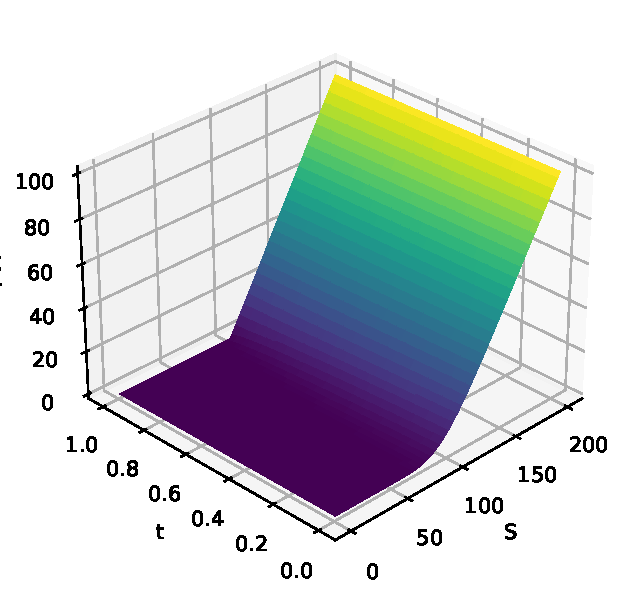
\includegraphics[width=\linewidth]{Imagenes/Parte1/6_Sols/Call/Call3D.pdf}
        \caption{Solución}
    \end{subfigure}
    \begin{subfigure}[b]{0.3\linewidth}
        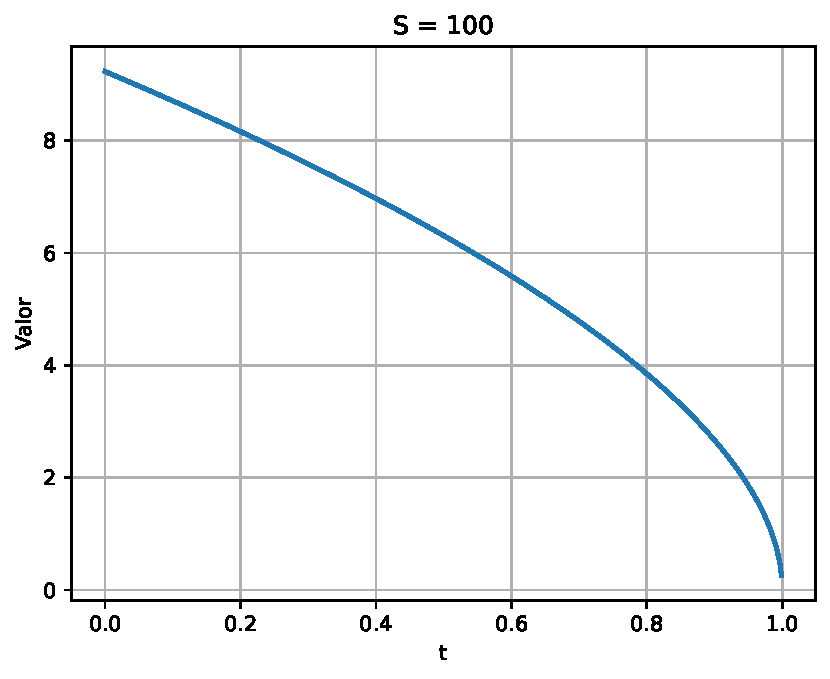
\includegraphics[width=\linewidth]{Imagenes/Parte1/6_Sols/Call/CallSFijo.pdf}
        \caption{Solución con S fijo}
    \end{subfigure}
    \begin{subfigure}[b]{0.3\linewidth}
        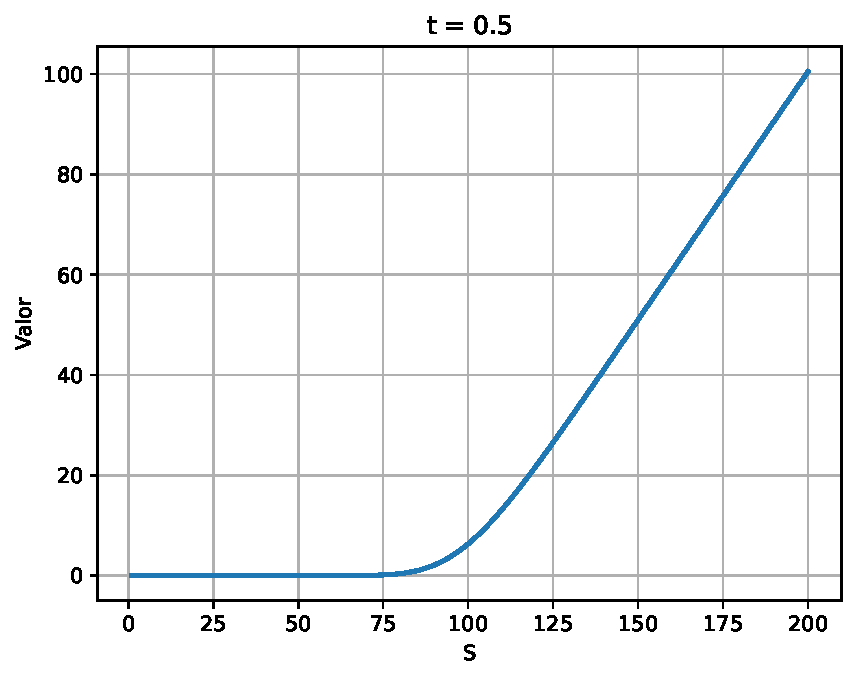
\includegraphics[width=\linewidth]{Imagenes/Parte1/6_Sols/Call/CalltFIjo.pdf}
        \caption{Solución con t fijo}
    \end{subfigure}
    \begin{subfigure}[b]{0.3\linewidth}
        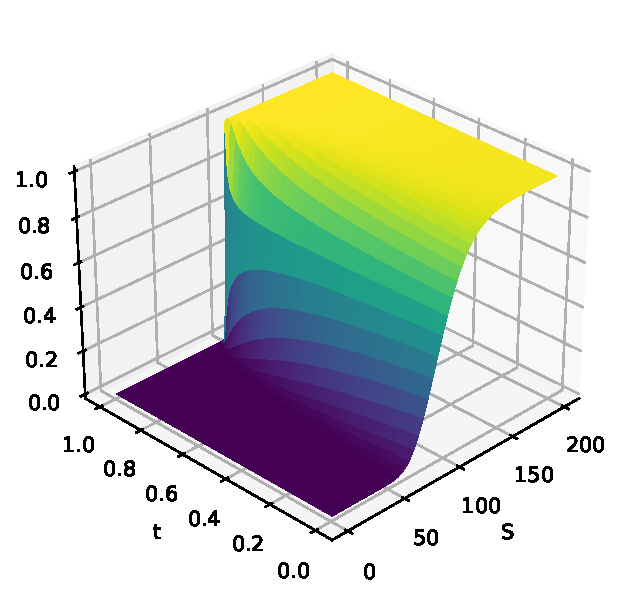
\includegraphics[width=\linewidth]{Imagenes/Parte1/6_Sols/Call/Call_Delta.pdf}
        \caption{Delta}
    \end{subfigure}
    \begin{subfigure}[b]{0.3\linewidth}
        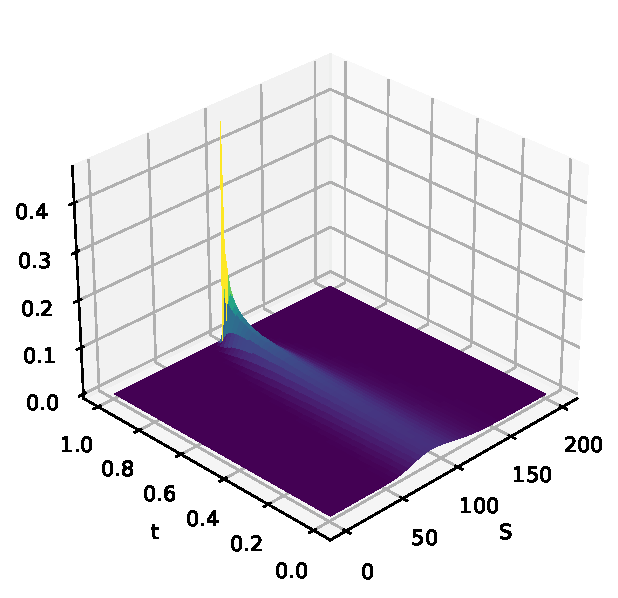
\includegraphics[width=\linewidth]{Imagenes/Parte1/6_Sols/Call/Call_Gamma.pdf}
        \caption{Gamma}
    \end{subfigure}
    \begin{subfigure}[b]{0.3\linewidth}
        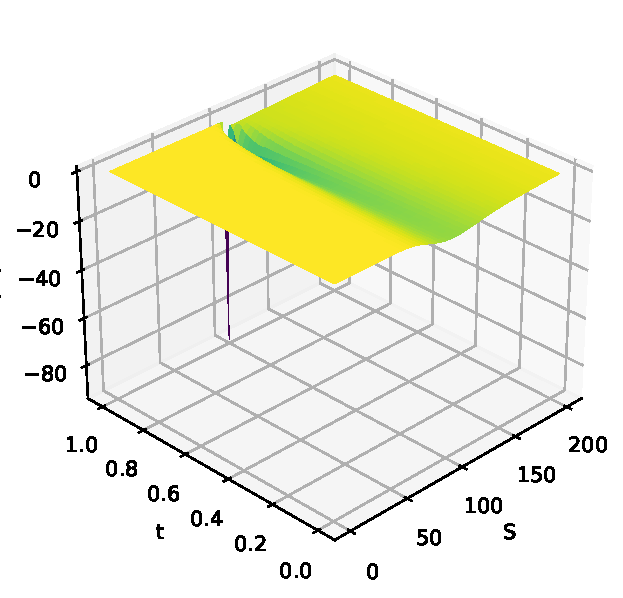
\includegraphics[width=\linewidth]{Imagenes/Parte1/6_Sols/Call/Call_Theta.pdf}
        \caption{Theta}
    \end{subfigure}
    \begin{subfigure}[b]{0.3\linewidth}
        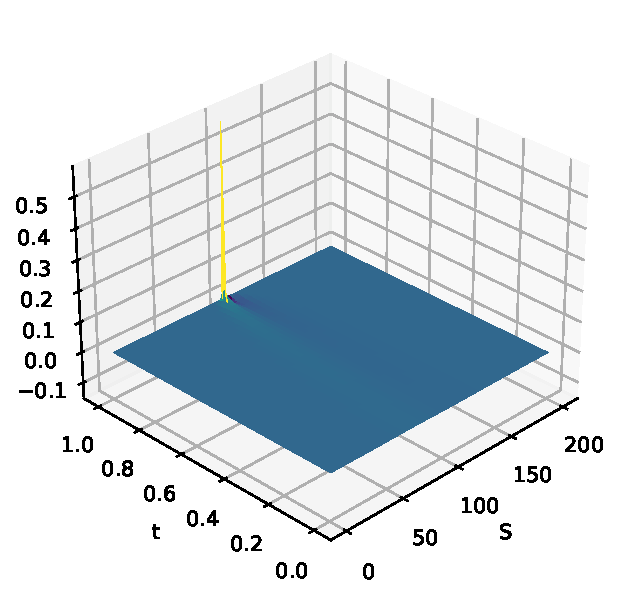
\includegraphics[width=\linewidth]{Imagenes/Parte1/6_Sols/Call/Call_Speed.pdf}
        \caption{Speed}
    \end{subfigure}
    \begin{subfigure}[b]{0.3\linewidth}
        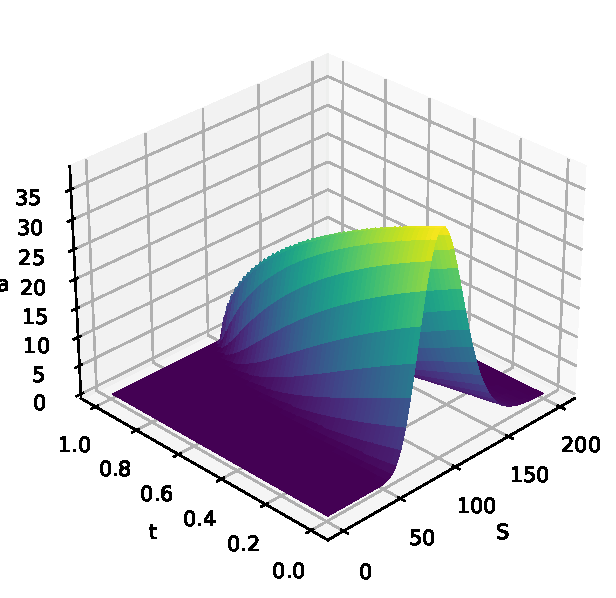
\includegraphics[width=\linewidth]{Imagenes/Parte1/6_Sols/Call/Call_Vega.pdf}
        \caption{Vega}
    \end{subfigure}
    \begin{subfigure}[b]{0.3\linewidth}
        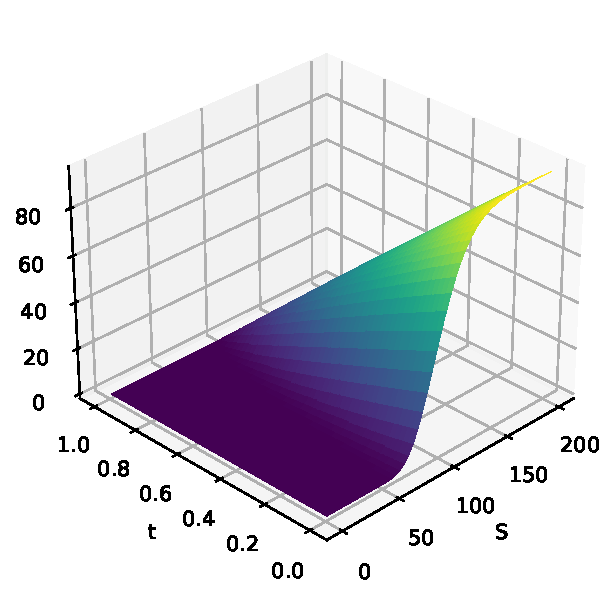
\includegraphics[width=\linewidth]{Imagenes/Parte1/6_Sols/Call/Call_Rho_r.pdf}
        \caption{Rho (r)}
    \end{subfigure}
    \begin{subfigure}[b]{0.3\linewidth}
        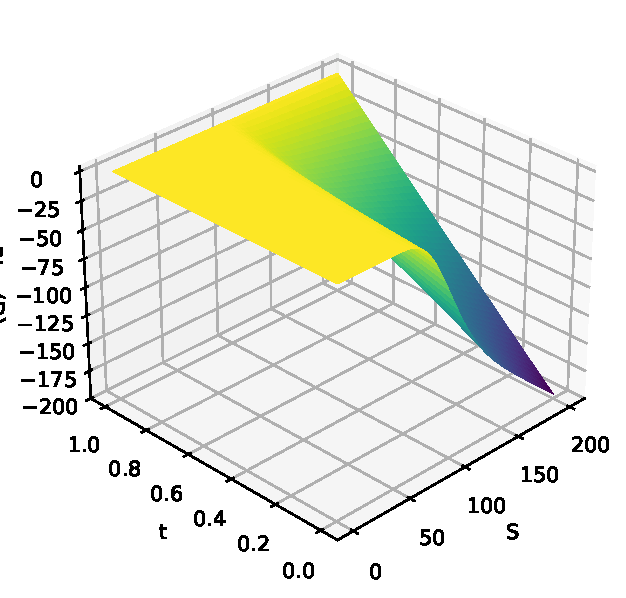
\includegraphics[width=\linewidth]{Imagenes/Parte1/6_Sols/Call/Call_Rho_D.pdf}
        \caption{Rho (D)}
    \end{subfigure}
\end{figure}


\subsubsection{Put option}
\begin{figure}[H]
    \centering
    \begin{subfigure}[b]{0.3\linewidth}
        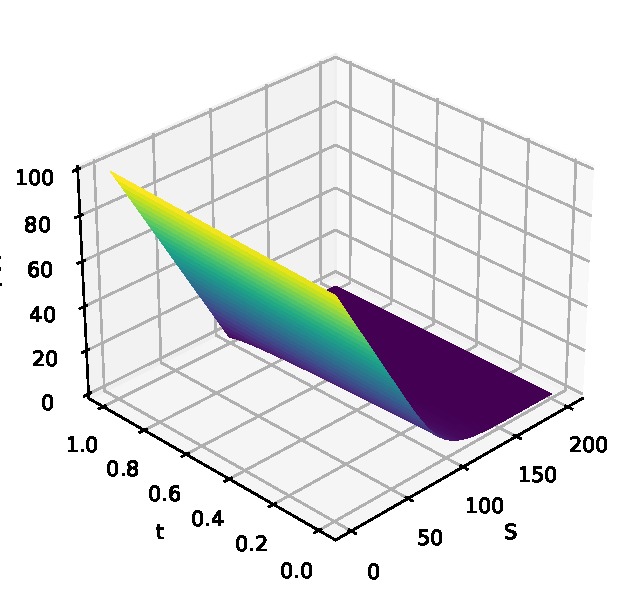
\includegraphics[width=\linewidth]{Imagenes/Parte1/6_Sols/Put/Put3D.pdf}
        \caption{Solución}
    \end{subfigure}
    \begin{subfigure}[b]{0.3\linewidth}
        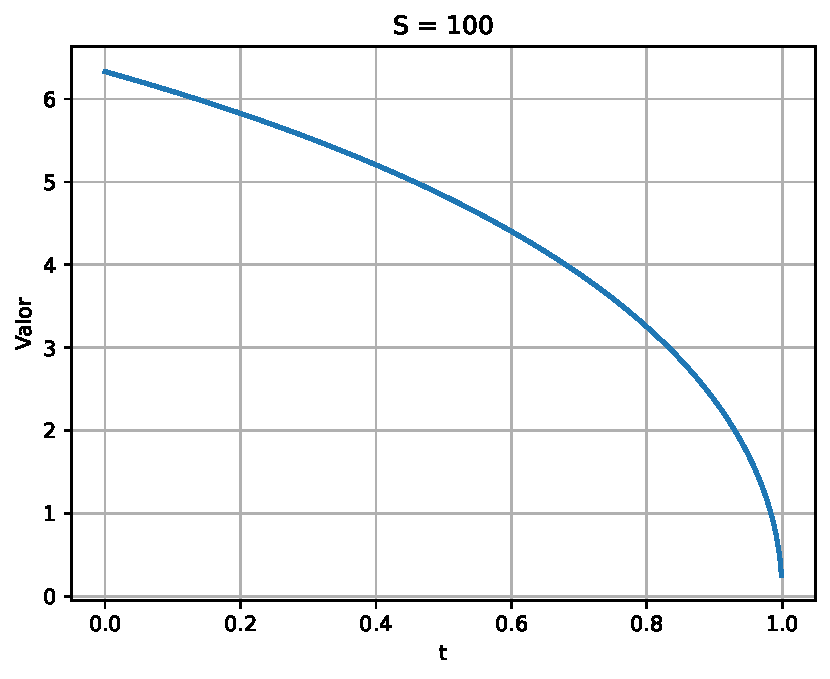
\includegraphics[width=\linewidth]{Imagenes/Parte1/6_Sols/Put/PutSFijo.pdf}
        \caption{Solución con S fijo}
    \end{subfigure}
    \begin{subfigure}[b]{0.3\linewidth}
        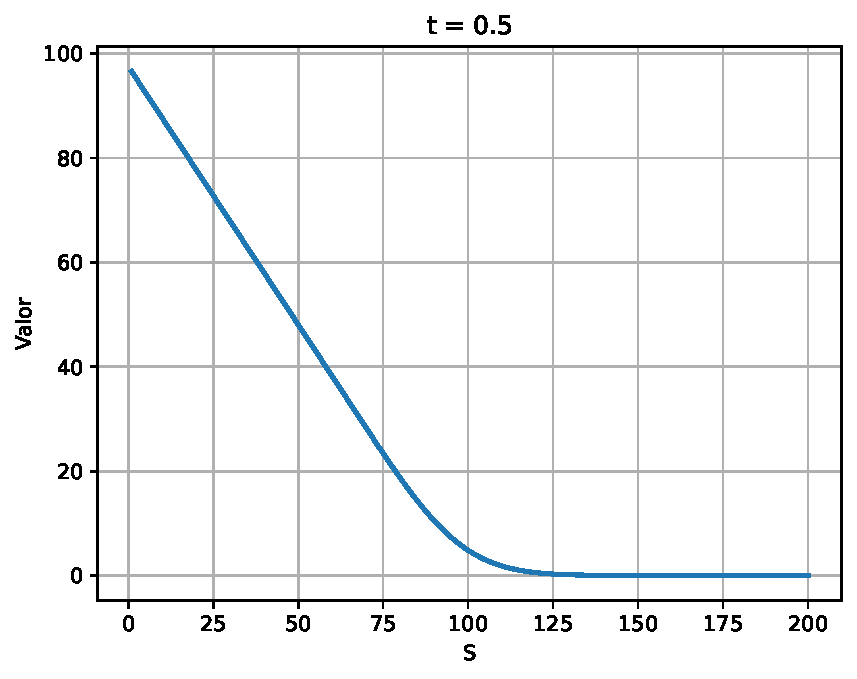
\includegraphics[width=\linewidth]{Imagenes/Parte1/6_Sols/Put/PuttFIjo.pdf}
        \caption{Solución con t fijo}
    \end{subfigure}
    \begin{subfigure}[b]{0.3\linewidth}
        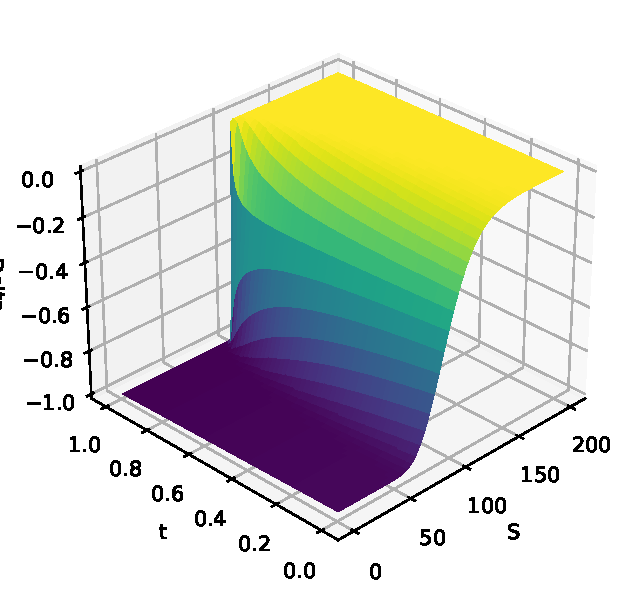
\includegraphics[width=\linewidth]{Imagenes/Parte1/6_Sols/Put/Put_Delta.pdf}
        \caption{Delta}
    \end{subfigure}
    \begin{subfigure}[b]{0.3\linewidth}
        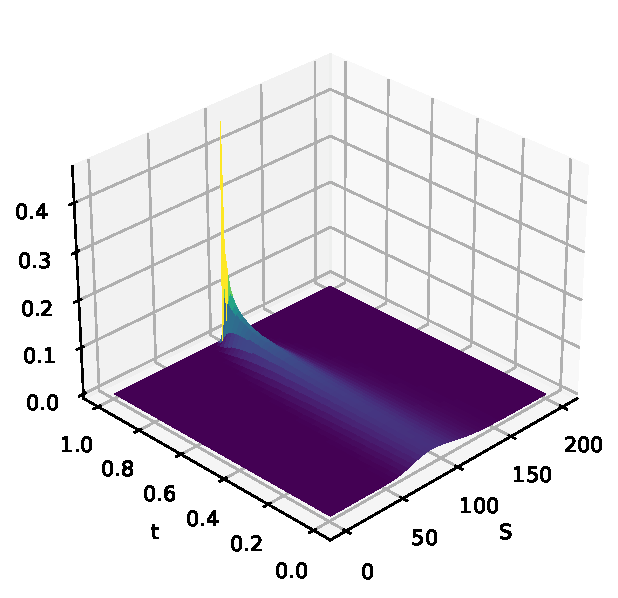
\includegraphics[width=\linewidth]{Imagenes/Parte1/6_Sols/Put/Put_Gamma.pdf}
        \caption{Gamma}
    \end{subfigure}
    \begin{subfigure}[b]{0.3\linewidth}
        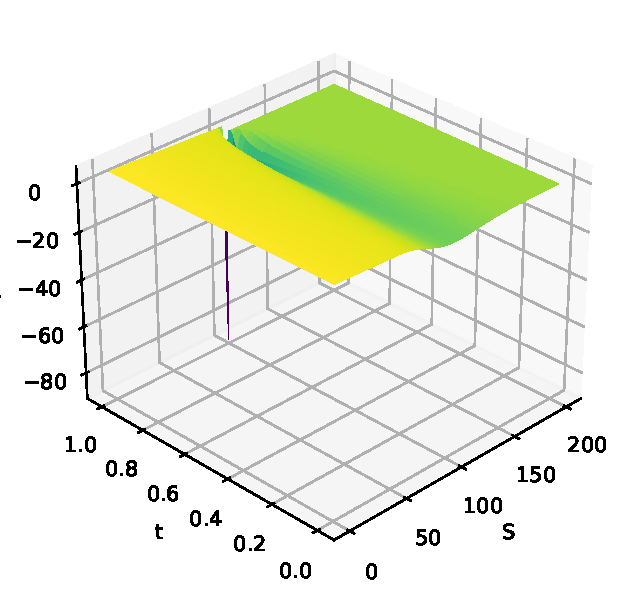
\includegraphics[width=\linewidth]{Imagenes/Parte1/6_Sols/Put/Put_Theta.pdf}
        \caption{Theta}
    \end{subfigure}
    \begin{subfigure}[b]{0.3\linewidth}
        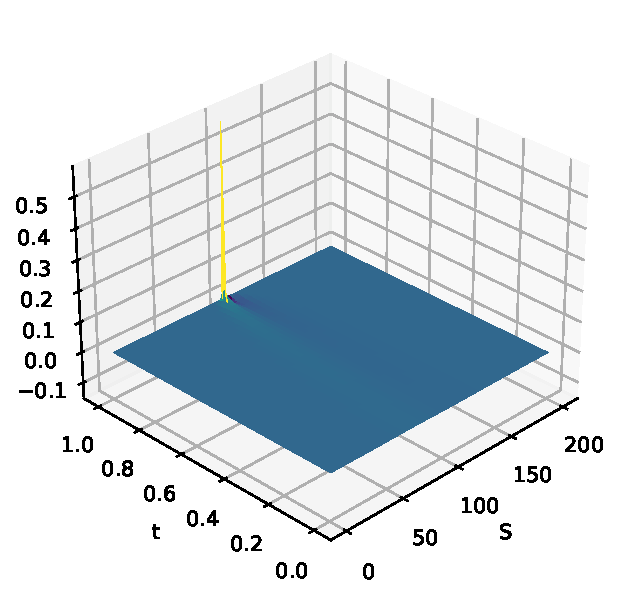
\includegraphics[width=\linewidth]{Imagenes/Parte1/6_Sols/Put/Put_Speed.pdf}
        \caption{Speed}
    \end{subfigure}
    \begin{subfigure}[b]{0.3\linewidth}
        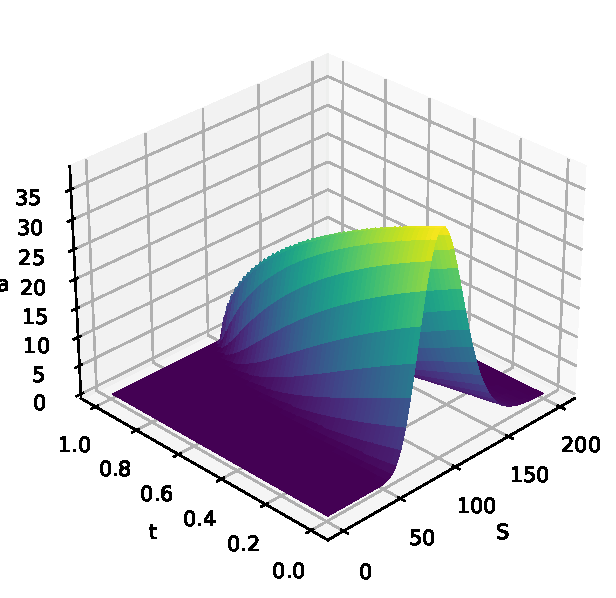
\includegraphics[width=\linewidth]{Imagenes/Parte1/6_Sols/Put/Put_Vega.pdf}
        \caption{Vega}
    \end{subfigure}
    \begin{subfigure}[b]{0.3\linewidth}
        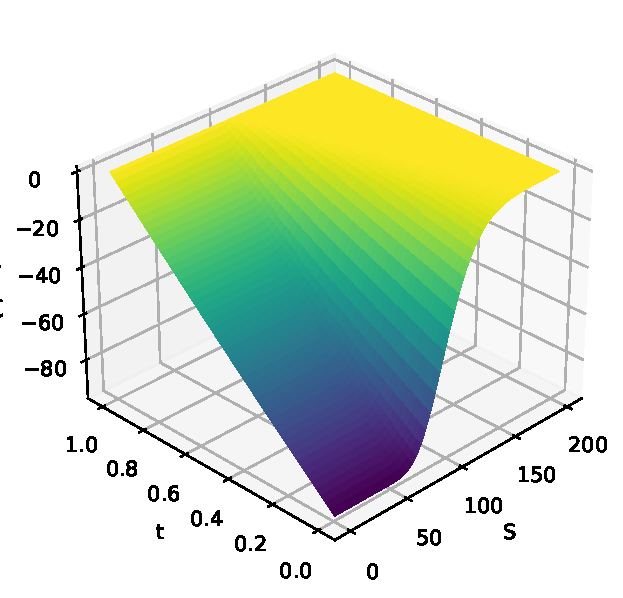
\includegraphics[width=\linewidth]{Imagenes/Parte1/6_Sols/Put/Put_Rho_r.pdf}
        \caption{Rho (r)}
    \end{subfigure}
    \begin{subfigure}[b]{0.3\linewidth}
        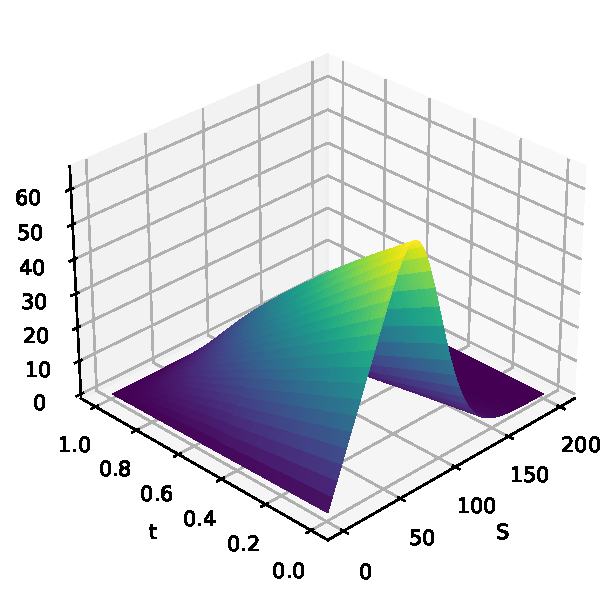
\includegraphics[width=\linewidth]{Imagenes/Parte1/6_Sols/Put/Put_Rho_D.pdf}
        \caption{Rho (D)}
    \end{subfigure}
\end{figure}



\subsubsection{Binary Call option}
\begin{figure}[H]
    \centering
    \begin{subfigure}[b]{0.3\linewidth}
        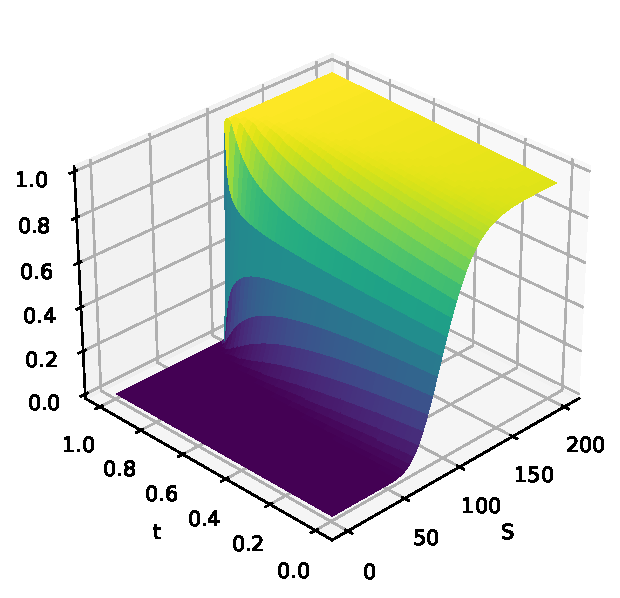
\includegraphics[width=\linewidth]{Imagenes/Parte1/6_Sols/Binary_Call/BinaryCall3D.pdf}
        \caption{Solución}
    \end{subfigure}
    \begin{subfigure}[b]{0.3\linewidth}
        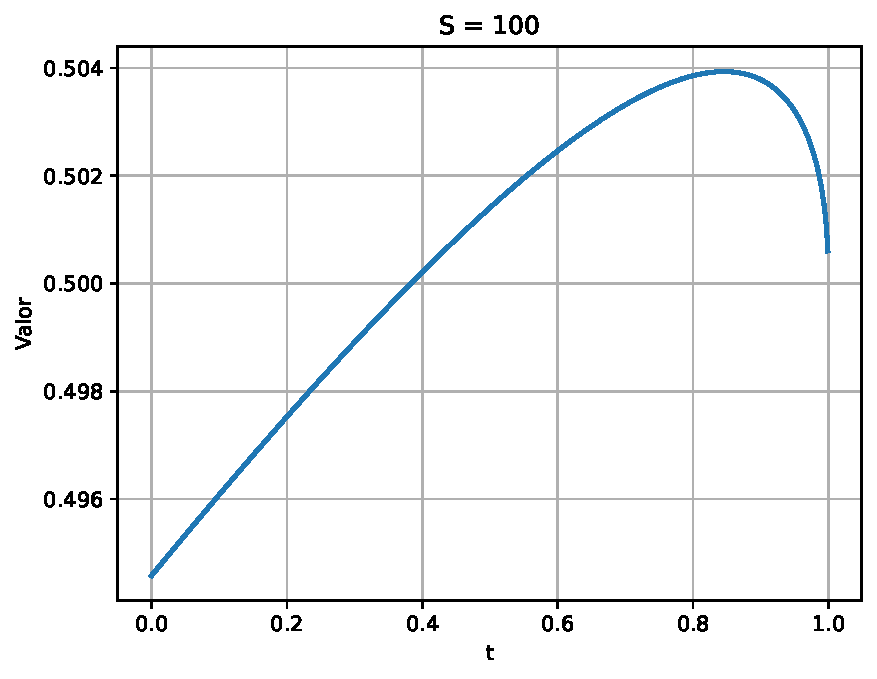
\includegraphics[width=\linewidth]{Imagenes/Parte1/6_Sols/Binary_Call/BinaryCallSFijo.pdf}
        \caption{Solución con S fijo}
    \end{subfigure}
    \begin{subfigure}[b]{0.3\linewidth}
        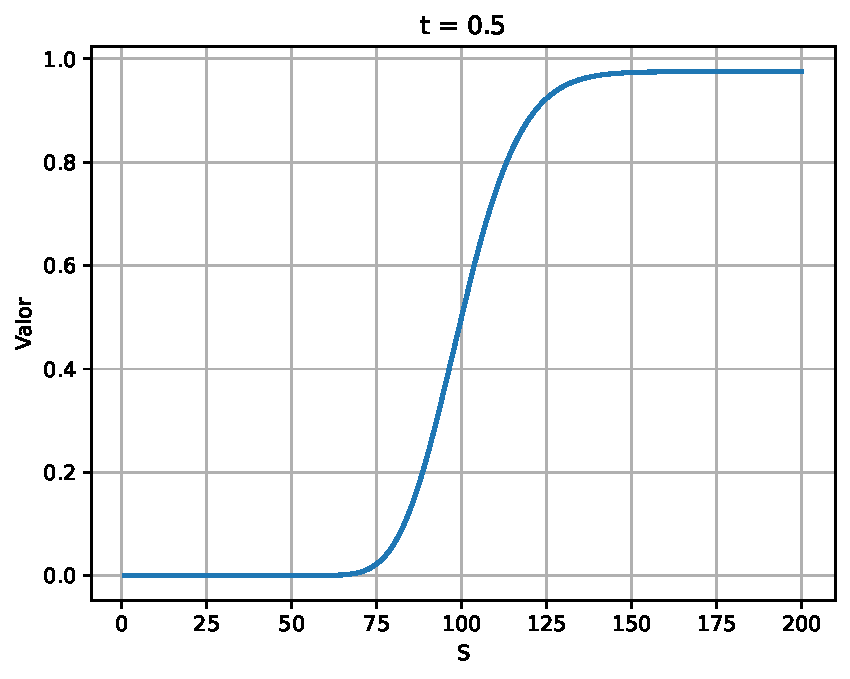
\includegraphics[width=\linewidth]{Imagenes/Parte1/6_Sols/Binary_Call/BinaryCalltFIjo.pdf}
        \caption{Solución con t fijo}
    \end{subfigure}
    \begin{subfigure}[b]{0.3\linewidth}
        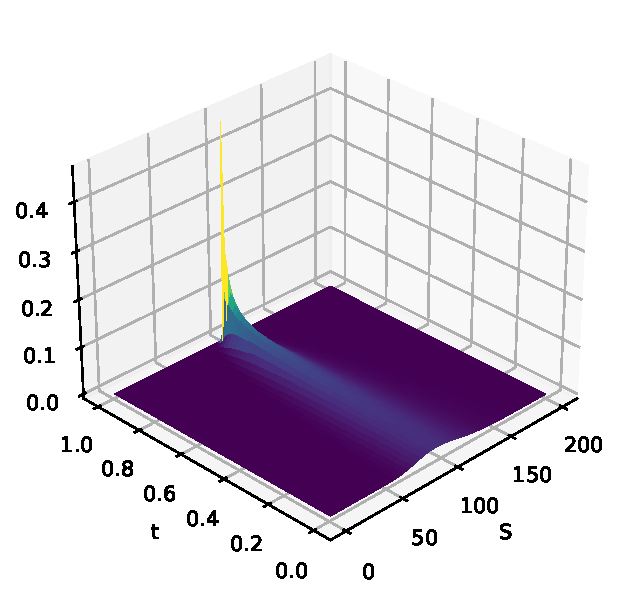
\includegraphics[width=\linewidth]{Imagenes/Parte1/6_Sols/Binary_Call/Binary_Call_Delta.pdf}
        \caption{Delta}
    \end{subfigure}
    \begin{subfigure}[b]{0.3\linewidth}
        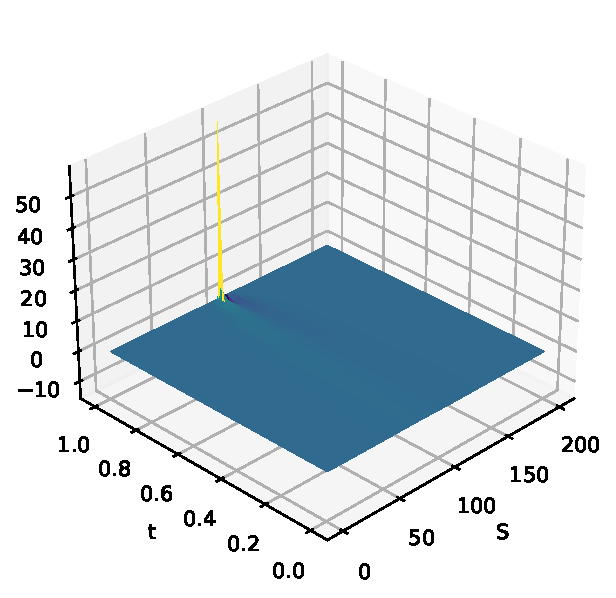
\includegraphics[width=\linewidth]{Imagenes/Parte1/6_Sols/Binary_Call/Binary_Call_Gamma.pdf}
        \caption{Gamma}
    \end{subfigure}
    \begin{subfigure}[b]{0.3\linewidth}
        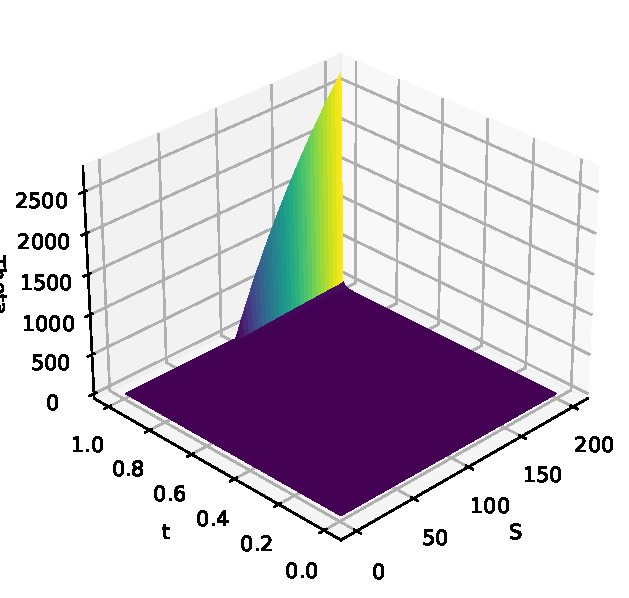
\includegraphics[width=\linewidth]{Imagenes/Parte1/6_Sols/Binary_Call/Binary_Call_Theta.pdf}
        \caption{Theta}
    \end{subfigure}
    \begin{subfigure}[b]{0.3\linewidth}
        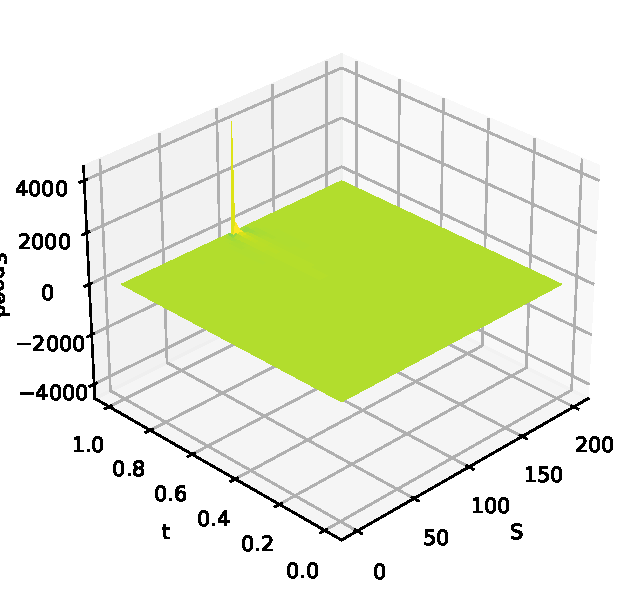
\includegraphics[width=\linewidth]{Imagenes/Parte1/6_Sols/Binary_Call/Binary_Call_Speed.pdf}
        \caption{Speed}
    \end{subfigure}
    \begin{subfigure}[b]{0.3\linewidth}
        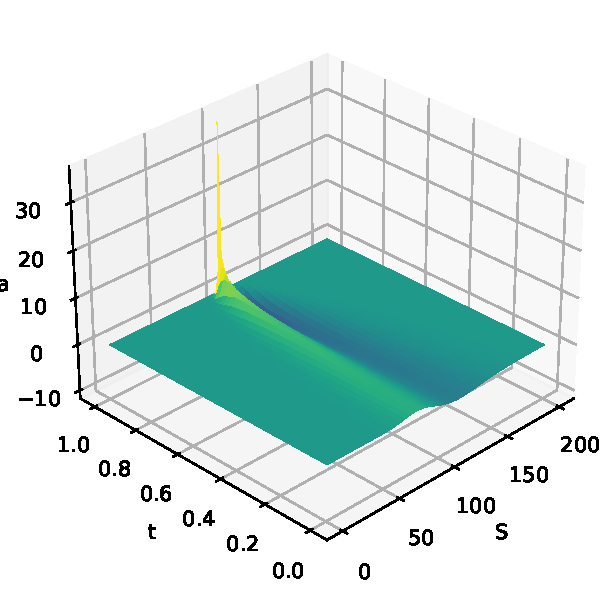
\includegraphics[width=\linewidth]{Imagenes/Parte1/6_Sols/Binary_Call/Binary_Call_Vega.pdf}
        \caption{Vega}
    \end{subfigure}
    \begin{subfigure}[b]{0.3\linewidth}
        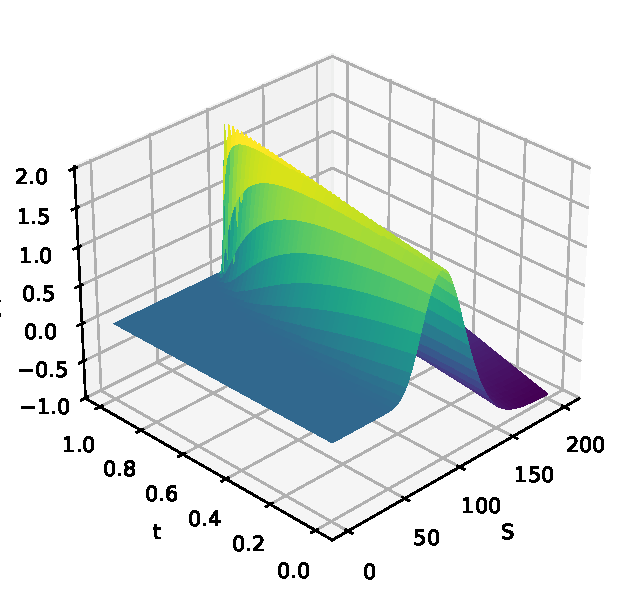
\includegraphics[width=\linewidth]{Imagenes/Parte1/6_Sols/Binary_Call/Binary_Call_Rho_r.pdf}
        \caption{Rho (r)}
    \end{subfigure}
    \begin{subfigure}[b]{0.3\linewidth}
        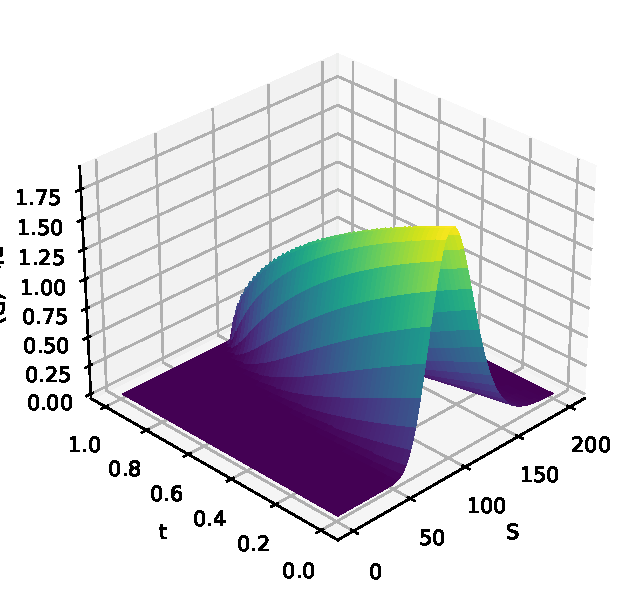
\includegraphics[width=\linewidth]{Imagenes/Parte1/6_Sols/Binary_Call/Binary_Call_Rho_D.pdf}
        \caption{Rho (D)}
    \end{subfigure}
\end{figure}


\subsubsection{Binary Put option}
\begin{figure}[H]
    \centering
    \begin{subfigure}[b]{0.3\linewidth}
        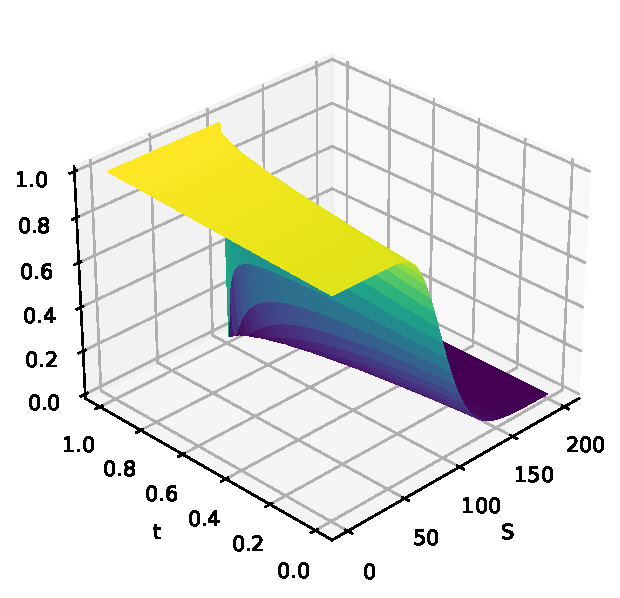
\includegraphics[width=\linewidth]{Imagenes/Parte1/6_Sols/Binary_Put/BinaryPut3D.pdf}
        \caption{Solución}
    \end{subfigure}
    \begin{subfigure}[b]{0.3\linewidth}
        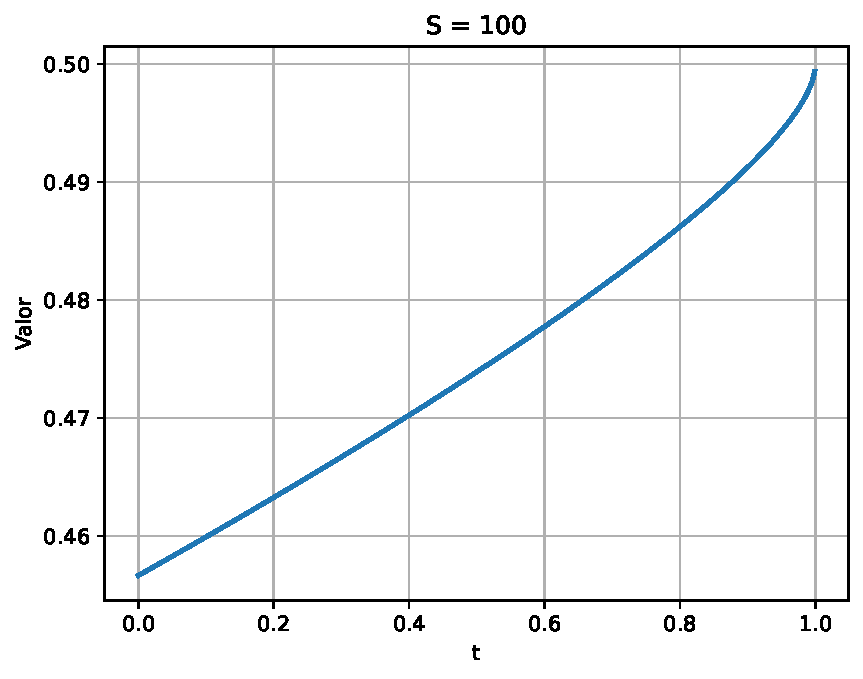
\includegraphics[width=\linewidth]{Imagenes/Parte1/6_Sols/Binary_Put/BinaryPutSFijo.pdf}
        \caption{Solución con S fijo}
    \end{subfigure}
    \begin{subfigure}[b]{0.3\linewidth}
        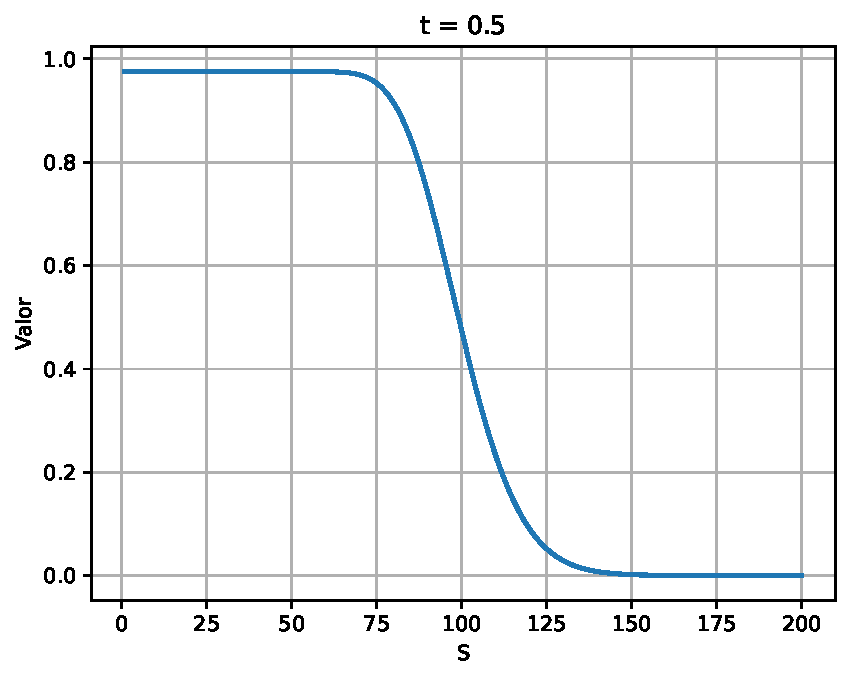
\includegraphics[width=\linewidth]{Imagenes/Parte1/6_Sols/Binary_Put/BinaryPuttFIjo.pdf}
        \caption{Solución con t fijo}
    \end{subfigure}
    \begin{subfigure}[b]{0.3\linewidth}
        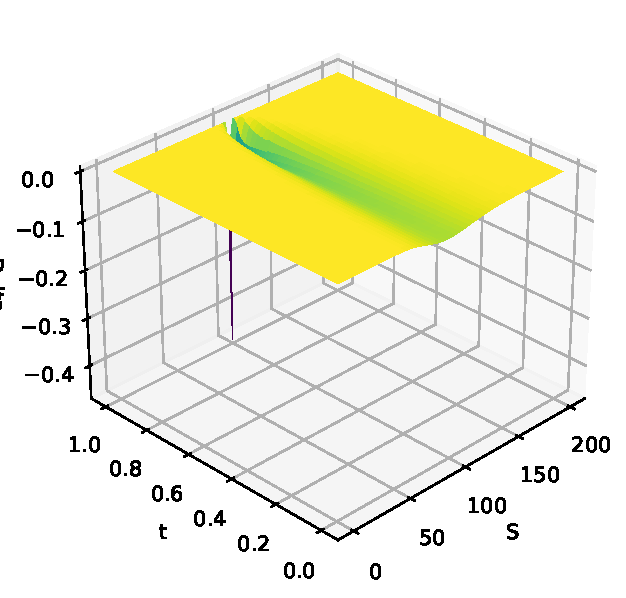
\includegraphics[width=\linewidth]{Imagenes/Parte1/6_Sols/Binary_Put/Binary_Put_Delta.pdf}
        \caption{Delta}
    \end{subfigure}
    \begin{subfigure}[b]{0.3\linewidth}
        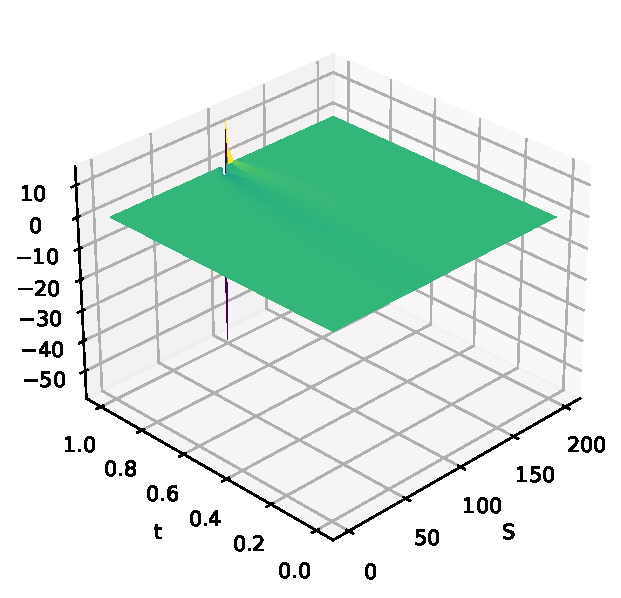
\includegraphics[width=\linewidth]{Imagenes/Parte1/6_Sols/Binary_Put/Binary_Put_Gamma.pdf}
        \caption{Gamma}
    \end{subfigure}
    \begin{subfigure}[b]{0.3\linewidth}
        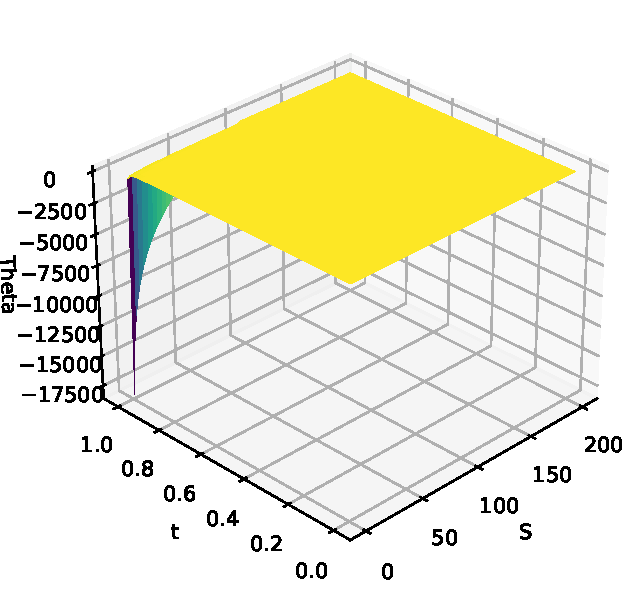
\includegraphics[width=\linewidth]{Imagenes/Parte1/6_Sols/Binary_Put/Binary_Put_Theta.pdf}
        \caption{Theta}
    \end{subfigure}
    \begin{subfigure}[b]{0.3\linewidth}
        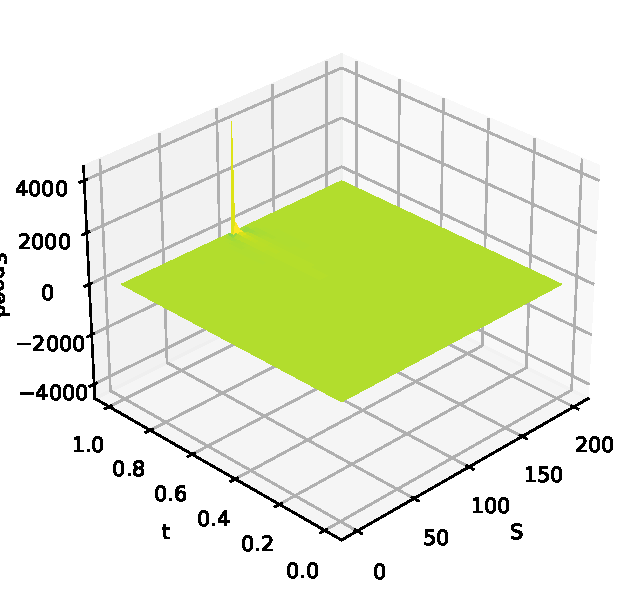
\includegraphics[width=\linewidth]{Imagenes/Parte1/6_Sols/Binary_Put/Binary_Put_Speed.pdf}
        \caption{Speed}
    \end{subfigure}
    \begin{subfigure}[b]{0.3\linewidth}
        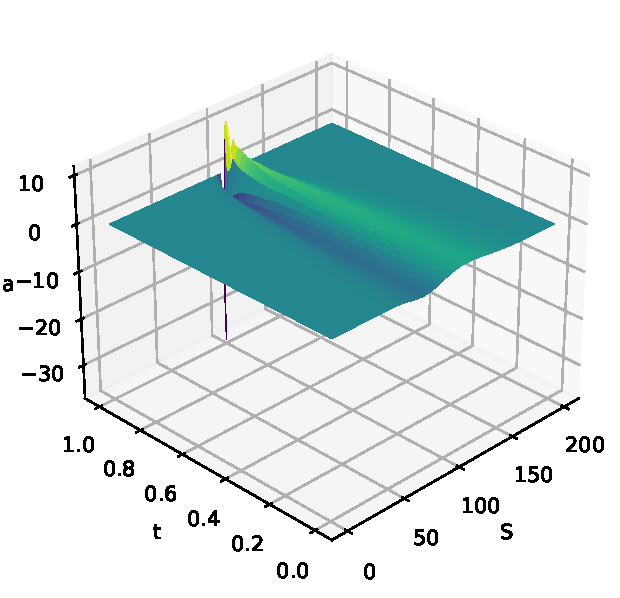
\includegraphics[width=\linewidth]{Imagenes/Parte1/6_Sols/Binary_Put/Binary_Put_Vega.pdf}
        \caption{Vega}
    \end{subfigure}
    \begin{subfigure}[b]{0.3\linewidth}
        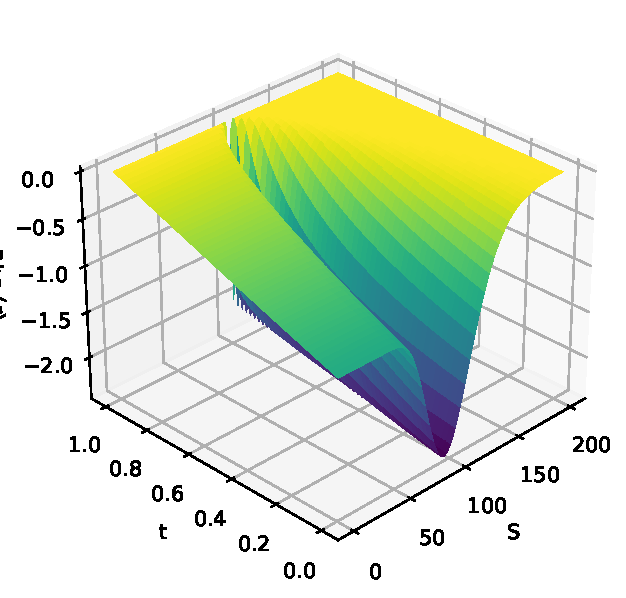
\includegraphics[width=\linewidth]{Imagenes/Parte1/6_Sols/Binary_Put/Binary_Put_Rho_r.pdf}
        \caption{Rho (r)}
    \end{subfigure}
    \begin{subfigure}[b]{0.3\linewidth}
        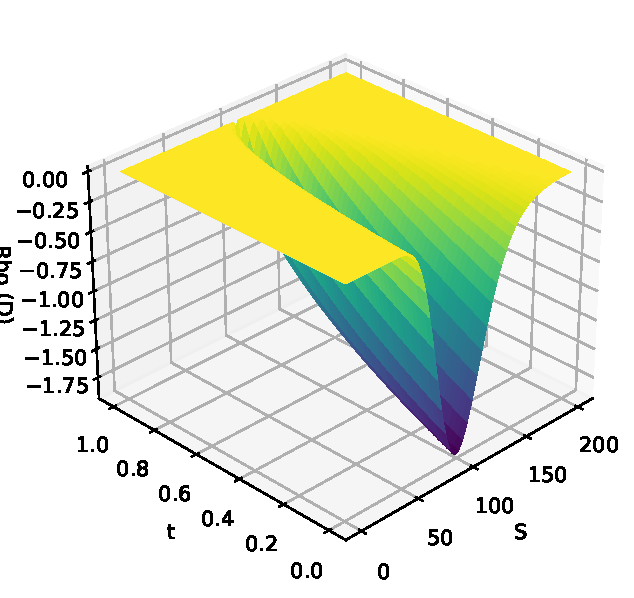
\includegraphics[width=\linewidth]{Imagenes/Parte1/6_Sols/Binary_Put/Binary_Put_Rho_D.pdf}
        \caption{Rho (D)}
    \end{subfigure}
\end{figure}





\subsection{Volatilidad implícita}\label{sec:vol_imp}
Valor de $\sigma$ que iguala precio teórico (Black-Scholes) al precio de mercado. Para su cálculo se utilizan métodos numéricos como Newton-Raphson usando vega.\\
No es consistente si se calcula para diferentes strikes y vencimientos, lo que genera distintas curvas de volatilidad implícita:
\begin{itemize}
    \item \textbf{Smile:} Volatilidad más alta para opciones ITM y OTM, mínima en ATM.\@
    \item \textbf{Skew:} Inclinación de la curva; típicamente negativa en mercados de acciones (mayor IV en puts OTM).
    \item \textbf{Frown:} Forma invertida del smile; menos común.
\end{itemize}





\subsection{Tipos de coberturas}
Según la independiencia con el modelo:
\begin{itemize}
    \item \textbf{Model-independent hedging:} Son pocos. No dependen de la dinámica del subyacente ni de la volatilidad. Por ejemplo la relación put-call parity.
    \item \textbf{Model-dependent hedging:} Son muchos más. Ejemplo más tipico es la cobertura usada en el análisis de Black-Scholes. Al valorar el derivado se necesita al menos la volatilidad.
\end{itemize}
Otros tipos de coberturas son:
\begin{itemize}
    \item \textbf{Delta hedging}: es la perfecta eliminación teórica del riesgo usando cobertura entre la opción y el subyacente. Es un ejemplo de cobertura \textbf{dinámica}: la cobertura se debe monitorizar y ajustar todo el rato, por lo que en la vida real va a dar lugar a pérdidas por los costes de transacción.
    \item \textbf{Gamma hedging}: usada para disminuir el tamaño de cada cobertura o para incrementar el tiempo entre coberturas (y así disminuir coste de transacción). Una cartera de este tipo es insensible a cambios del subyacente mientras sean movimientos pequeños. 
    \item \textbf{Vega hedging}: usada para eliminar el riesgo de volatilidad. En realidad esto en ocasiones da lugar a inconsistencias y no se debe usar una volatilidad constante.
    \item \textbf{Static hedging}: usada para reducir el riesgo de opciones exóticas mediante contratos más líquidos que se mantienen hasta el vencimiento, eliminando la necesidad de ajustes dinámicos.
    \item \textbf{Margin hedging}: usada para equilibrar las llamadas de margen (depósitos obligatorios) en una parte del portafolio con los reembolsos de otras partes, evitando así grandes llamadas de margen que puedan ser difíciles de cumplir.
    \item \textbf{Crash (Platinum) hedging}: diseñada para minimizar el peor resultado posible en mercados extremos (p.e.\ caídas), donde los movimientos son tan grandes que no se puede seguir el ritmo con las coberturas, y además las correlaciones normales se vuelven irrelevantes. Incluye dos tipos: cobertura del valor nominal del portafolio y cobertura de llamadas de margen.
\end{itemize}






